\chapter{Il livello di rete}
\label{cap:livelloRete}
\thispagestyle{chapterInit}
\section{Visione d'insieme}
    \paragraph{Obbiettivo del livello di rete} L'obbiettivo principale del livello di rete è quello di permettere la comunicazione tramite reti diverse attraverso apparecchi detti \textit{router} i quali hanno il compito di inoltrare le informazioni verso la destinazione.
    \paragraph{Funzioni principali} Esistono due funzioni principali del livello di rete: \begin{description}
        \item[Inoltro \textit{forwarding}] Questa è una operazione a livello locale che consiste nel prendere un pacchetto in ingresso e inoltrarlo verso l'uscita corretta.
        \item[Instradamento \textit{routing}] Questa è una operazione a livello globale che consiste nel determinare il percorso migliore per inoltrare un pacchetto verso la destinazione. Per questa operazione si utilizzano degli algoritmi di \textit{routing}.
    \end{description}
    Queste due funzioni sono legate tra loro, ma possono essere isolate. Infatti convenzionalmente distinguiamo con \textit{control plane} la parte del livello di rete che si occupa dell'istradamento e con \textit{data plane} la parte che si occupa dell'inoltro. Questa distinzione è utile per capire come funzionano i router.
    \subparagraph{\textit{Data Pane}} Il \textit{data plane} ha funzione a livello locale ad ogni \textit{router}, questo è il livello che determina \underline{come} inoltrare un \textit{datagram} fornendo la funzione di \textit{forwarding}.
    \subparagraph{\textit{Control Plane}} Il \textit{control plane} ha funzione a livello globale, questo è il livello che determina \underline{dove} inoltrare un \textit{datagram} fornendo la funzione di \textit{routing}.
\section{Come è fatto un router}
    Visto a livello "alto" un router è composto da tre livelli principali: \begin{description}
        \item[Terminazione di linea] Questo è il livello più basso del router, è composto da un'interfaccia di rete che si occupa di ricevere i pacchetti e di inviarli al livello successivo.
        \item[Protocollo di livello \textit{data link}] Questo livello si occupa di ricevere i pacchetti dal livello precedente e di inviarli al livello successivo. Inoltre si occupa di fare il controllo degli errori e di gestire il flusso.
        \item[Inoltro e \textit{buffer}] Questo è il livello che si occupa di inoltrare i pacchetti verso la destinazione. Inoltre si occupa di fare il \textit{buffering} dei pacchetti in caso di congestione.
    \end{description}
    \subsection{Sistemi di commutazione}
        I sistemi di commutazione trasferiscono i pacchetti dalle porte di ingresso all'uscita appropriata. Definiamo come \textbf{tasso di comunicazione} la frequenza alla quale i pacchetti vengono portati dall'ingresso all'uscita (spesso è un multiplo della velocità di comunicazione) 
        \subsubsection{Commutazione a memoria}
            Questo è il metodo più semplice, i pacchetti vengono memorizzati in un buffer comune e poi inoltrati verso l'uscita appropriata. Questo metodo è molto semplice ma ha il problema che la velocità di inoltro è limitata dalla velocità di accesso alla memoria.
        \subsubsection{Commutazione a bus}
            Questo metodo consiste nel collegare le porte di ingresso e di uscita tramite un bus, sempre comune a tutte le porte. Questo metodo risulta lento in quanto non possono essere trasferiti più pacchetti contemporaneamente anche se le porte di ingresso e di uscita sono diverse. Il \texttt{Cisco 5600} è un esempio di router che utilizza questo metodo e riesce a trasferire fino a 32 Gbit/s.
        \subsubsection{Commutazione a matrice}
            Questo metodo consiste nel collegare le porte di ingresso e di uscita tramite una matrice di commutazione. Questo metodo è molto veloce in quanto permette di trasferire più pacchetti contemporaneamente in quanto se le porte sono differenti allora basta attivare i vari collegamenti della matrice. Questo metodo è molto veloce ed ispirato ai primi commutatori telefonici. Il \texttt{Cisco 12000} è un esempio di router che utilizza questo metodo e riesce a trasferire fino a 60 Gbit/s.
    \subsection{Accodamenti}
        Gli accodamenti sono utilizzati per evitare la perdita di pacchetti in caso di congestione dell'apparecchio di rete. Questo è un problema molto comune in quanto i router sono dispositivi molto veloci e le porte di uscita sono molto più lente. Per evitare la perdita di pacchetti si utilizzano delle code che permettono di memorizzare i pacchetti in attesa di essere inoltrati.
        Le code possono essere formate in ingresso, quando una stessa porta di uscita è condivisa da più porte di ingresso e quindi una porta di uscita può essere congestionata. Le code possono essere formate in uscita, quando una porta di uscita ha un \textit{link} più lento rispetto alla velocità di inoltro dei pacchetti tramite le porte di ingresso o il commutatore di pacchetto.
        \paragraph{Quanta memoria serve per i \textit{buffer}} Secondo \texttt{RFC 3439} la quantità di memoria necessaria per i buffer è data dalla formula: \[M = \frac{RTT \cdot C}{\sqrt{N}}\] Dove: \begin{description}
            \item[$M$] è la memoria necessaria per il buffer
            \item[$RTT$] è il tempo di round trip
            \item[$C$] è la capacità del collegamento
            \item[$N$] è il numero di connessioni
        \end{description}
        \paragraph{Meccanismi di \textit{scheduling}}
            I meccanismi di \textit{scheduling} sono utilizzati per decidere quale pacchetto inoltrare quando si ha la possibilità di inoltrare più pacchetti. Il meccanismo più semplice è il \textit{First In First Out} (\texttt{FIFO}) che inoltra i pacchetti in ordine di arrivo. Inoltre viene applicata una politica di scarto dei pacchetti in caso di buffer pieno. Questa politica può essere: \begin{description}
                \item[\textit{Drop Tail}] Questa politica scarta i pacchetti in arrivo quando il buffer è pieno.
                \item[\textit{Random Early Detection}] Questa politica scarta i pacchetti in arrivo in modo casuale quando il buffer è pieno.
                \item[\textit{Priority Drop}] Questa politica scarta i pacchetti in arrivo in base alla priorità.
            \end{description}
            La politica di scarto dei pacchetti dipende dall'implementazione del router.
\section{Il protocollo \texttt{IP}}
    \subsection{Il formato del \textit{datagram} \texttt{IP} (\texttt{IPv4})}
        \begin{figure}[H]
            \centering
            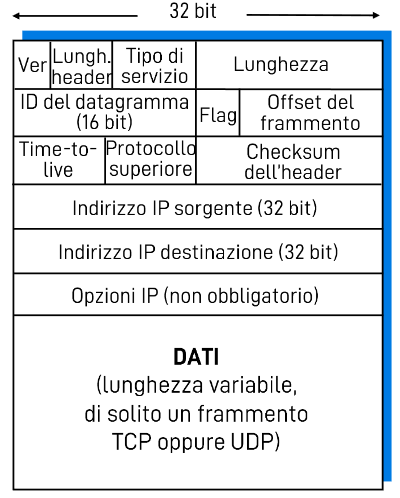
\includegraphics[width=0.36\textwidth]{04/datagramIPv4.png}
            \caption{Il formato del \textit{datagram} \texttt{IP} (\texttt{IPv4})}
            \label{fig:IPv4Header}
        \end{figure}
        Il formato del \textit{datagram} \texttt{IP} è composto da 20 byte di intestazione e da un campo dati. Il campo dati può contenere fino a 65.535 byte.  Di seguito si riportano i vari campi dell'intestazione:
        \begin{description}
            \item[VER] (4 bit) Questo campo contiene la versione del protocollo \texttt{IP} utilizzato.
            \item[Lunghezza \textit{header}] (4 bit) Questo campo contiene la lunghezza dell'intestazione in parole da 32 bit. (=5 se non ci sono opzioni)
            \item[Tipo di servizio - \texttt{ToS}] (8 bit) Questo campo contiene informazioni sul tipo di servizio richiesto.
            \item[Lunghezza totale] (16 bit) Questo campo contiene la lunghezza totale del \textit{datagram} in byte.
            \item[Identificativo] (16 bit) Questo campo contiene un numero univoco per il \textit{datagram}.
            \item[Flag] (3 bit) Questo campo contiene i flag per il frammento. Il primo bit è il bit di \textit{Don't Fragment}, il secondo bit è il bit di \textit{More Fragment} e il terzo bit è il bit di \textit{Fragment Offset}.
            \item[Offset] (13 bit) Questo campo contiene l'offset del frammento. (Espresso in multipli di 8 byte)
            \item[\textit{Time To Live} - \texttt{TTL}] (8 bit) Questo campo contiene il numero di \textit{hop} massimo che il \textit{datagram} può fare.
            \item[Protocollo] (8 bit) Questo campo contiene il protocollo di trasporto che si trova nel campo dati.
            \item[Checksum] (16 bit) Questo campo contiene il checksum dell'intestazione.
            \item[Indirizzo IP sorgente] (32 bit) Questo campo contiene l'indirizzo IP sorgente.
            \item[Indirizzo IP destinazione] (32 bit) Questo campo contiene l'indirizzo IP destinazione.
            \item[Opzioni] (variabile) Questo campo contiene le opzioni del \textit{datagram}.
            \item[Padding] (variabile) Questo campo contiene il padding per allineare l'intestazione a multipli di 32 bit.
        \end{description}
    \subsection{\texttt{MTU} e Frammentazione}
        La \texttt{MTU} (\textit{Maximum Transmission Unit}) è la dimensione massima di un pacchetto che può essere trasmesso su un collegamento, ogni \textit{hardware} specifica il proprio \texttt{MTU}. Se un \textit{datagram} è più grande della \texttt{MTU} allora il \textit{datagram} viene frammentato in pacchetti più piccoli. Questo processo è chiamato \textit{frammentazione}. I pacchetti frammentati vengono poi ricomposti alla destinazione.
        \paragraph{Valori Standard \texttt{MTU}} Per alcuni tipi di collegamenti sono stati definiti dei valori standard di \texttt{MTU}. Ad esempio per le reti Ethernet la \texttt{MTU} è di $1500$ byte, per le reti \texttt{WLAN 802.11} la \texttt{MTU} è di $2304$ byte,\dots. In un collegamento tra due \textit{host} possono essere presenti due valori di \texttt{MTU} diversi
        \subparagraph{Esempio} Supponendo che per raggiungere un host \texttt{B} si debba passare prima da una rete con $1500$ byte di \texttt{MTU} e poi da una rete con $1000$, tutto ciò tramite un router \texttt{R}. Allora quando il \textit{router} \texttt{R} riceve il datagram di $1500$ byte lo frammenta in due pacchetti di $1000$ byte e $500$ byte. I pacchetti vengono quindi inoltrati alla destinazione. Quando l'host \texttt{B} riceve i pacchetti li ricomponi e li passa al livello di trasporto.
        
    \subsection{Indirizzamento e \texttt{NAT}}
        \subsubsection{Indirizzi \texttt{IP}}
            Un indirizzo \texttt{IP} è composto da $32$ bit ed è associato ad un'interfaccia di rete. Una interfaccia è una connessione tramite mezzo fisico o logico, solitamente ogni \textit{host} ha una o più interfacce di rete.
            \paragraph{Caratteristiche indirizzi \texttt{IP}} Gli host e i router devono usare le stesse convenzioni per gli indirizzi \texttt{IP}, inoltre ogni indirizzo \texttt{IP} deve essere unico e raggiungibile da un qualsiasi punto di internet. Quando si invia un pacchetto \texttt{IP} si invia l'indirizzo \texttt{IP} sorgente e l'indirizzo \texttt{IP} destinazione. I \textit{router} sono apparati di rete che quando ricevono un pacchetto \texttt{IP} decidono dove inoltrarlo in base all'indirizzo \texttt{IP} di destinazione.
            \paragraph{Norazione indirizzo \texttt{IP}} Gli indirizzi \texttt{IP} sono composti da $4$ gruppi di $8$ bit e sono scritti in notazione decimale a punti. Ogni gruppo di $8$ bit è espresso in decimale e separato da un punto. Gli indirizzi disponibili vanno dà: $0.0.0.0$ a $255.255.255.255$ 
            \paragraph{Gerarchie indirizzi \texttt{IP}} Gli indirizzi \texttt{IP} sono organizzati in una struttura gerarchica. Inoltre solitamente sono divisi in due parti: \begin{description}
                \item[Parte di rete] Questa parte identifica la rete a cui appartiene l'indirizzo \texttt{IP}.
                \item[Parte di \textit{host}] Questa parte identifica l'\textit{host} all'interno della rete.
            \end{description}
            \subparagraph{Classi di indirizzi \texttt{IP}} Gli indirizzi \texttt{IP} sono divisi in classi sulla base dei primi bit dell'indirizzo e dalla lunghezza del prefisso: \begin{description}
                \item[Classe \texttt{A}] Gli indirizzi di classe \texttt{A} hanno il primo bit a \texttt{0} e sono composti da $8$ bit di rete e $24$ bit di \textit{host}. Gli indirizzi vanno da $0.0.0.0$ a $ 127.255.255.255$ e sono riservati per le reti molto grandi.
                \item[Classe \texttt{B}] Gli indirizzi di classe \texttt{B} hanno i primi due bit a \texttt{10} e sono composti da $16$ bit di rete e $16$ bit di \textit{host}. Gli indirizzi vanno da $128.0.0.0$ a $191.255.255.255$ e sono riservati per le reti di medie dimensioni.
                \item[Classe \texttt{C}] Gli indirizzi di classe \texttt{C} hanno i primi tre bit a \texttt{110} e sono composti da $24$ bit di rete e $8$ bit di \textit{host}. Gli indirizzi vanno da $192.0.0.0$ a $223.255.255.255$ e sono riservati per le reti di piccole dimensioni.
                \item[Classe \texttt{D}] Gli indirizzi di classe \texttt{D} hanno i primi quattro bit a \texttt{1110} e sono riservati per i \textit{multicast}.
                \item[Classe \texttt{E}] Gli indirizzi di classe \texttt{E} hanno i primi quattro bit a \texttt{1111} e sono riservati per usi futuri.
            \end{description}
        \subsubsection{Assegnazione indirizzi \texttt{IP}}
            Gli indirizzi \texttt{IP} sono assegnati dalla \texttt{ICANN} (\textit{Internet Corporation for Assigned Names and Numbers}) che riserva una intera classe ai \texttt{ISP} (\textit{Internet Service Provider}) e poi questi assegnano gli indirizzi ai propri clienti. Gli indirizzi \texttt{IP} sono assegnati in modo gerarchico e quindi un \texttt{ISP} può assegnare un intero blocco di indirizzi ad un altro \texttt{ISP} e questo può assegnare un blocco di indirizzi ad un altro \texttt{ISP} e così via.
    \subsection{Indirizzamento \textit{classless}}
        In quanto ci si è accorti che con la suddivisione degli indirizzi in classi si stava sprecando molti indirizzi, si è deciso di passare ad un indirizzamento \textit{classless}. Questo tipo di indirizzamento permette di avere una suddivisione più flessibile degli indirizzi, in quanto possiamo richiedere al nostro \texttt{ISP} solo un \textit{range} di indirizzi e non una classe intera, ad esempio l'\texttt{ISP} può usare un prefisso di $26$ bit per identificare la rete nel mondo e successivamente usare i restanti $6$ bit per identificare tutti gli \textit{host} della rete.
        In questa situazione se un \texttt{ISP} ha acquistato una rete di classe \texttt{C} e ha bisogno di dividere la rete in quattro clienti allora può dividere la rete in $4$ sotto-reti e assegnare un prefisso di $26$ bit ($24$ per la classe \texttt{C} e $2$ per le sotto-reti) e i restanti $6$ bit per gli \textit{host} di ogni sotto-rete.
        \subsubsection{Maschere di rete}
            In quanto ora non si ha più una suddivisione fissa degli indirizzi, si è deciso di introdurre le \textit{maschere di rete}. Queste maschere sono composte da $32$ bit e sono composte da una parte di $1$ quelli che identificano il prefisso di rete e da una parte di $0$ che identificano gli \textit{host} della rete. Ad esempio la maschera di rete per una rete di classe \texttt{C} è $11111111.11111111.11111111.00000000$.
            \paragraph{Peché si usa?} La maschera di rete viene usata per identificare la rete di appartenenza di un indirizzo IP. Per fare ciò si fa un'operazione di \texttt{AND} tra l'indirizzo IP di destinazione e la maschera di rete. Se il risultato è uguale all'indirizzo di rete allora l'indirizzo IP appartiene alla rete. Quindi se il prefisso di rete è $128.10.0.0$ ovvero: \[10000000.00001010.00000000.00000000\] e la maschera di rete è $255.255.0.0$ ovvero: \[11111111.11111111.00000000.00000000\] e l'indirizzo IP di destinazione di un determinato pacchetto è: $128.10.2.3$ ovvero: \[10000000.00001010.00000010.00000011\] allora facendo l'operazione di \texttt{AND} tra l'indirizzo IP e la maschera di rete si ottiene: \[\begin{aligned}
                10000000.00001010.00000010.00000011 &\\
                11111111.11111111.00000000.00000000 &\\
                \hline
                10000000.00001010.00000000.00000000&=128.10.0.0
            \end{aligned}
            \] Quindi l'indirizzo IP appartiene alla rete e il pacchetto viene inoltrato a quella determinata porta di uscita.
        \subsubsection{Notazioni \texttt{CIDR}}
            \texttt{CIDR} o \textit{Classless Inter-Domain Routing} è un metodo per rappresentare le maschere di rete. Questo metodo consiste nel rappresentare la maschera di rete con un prefisso di bit. Ad esempio la maschera di rete $/24$ è uguale alla maschera di rete $11111111.11111111.11111111.00000000$, ovvero una maschera di rete di classe \texttt{C}, quindi i primi $3$ gruppi di bit sono appartenenti all'\textit{network-id} e l'ultimo gruppo di bit è appartenente all'\textit{host-id}. La notazione prevede inoltre che gli indirizzi \texttt{IP} siano rappresentati nel seguente modo: \texttt{ddd.ddd.ddd.ddd/m} dove ogni singolo \texttt{d} rappresenta un gruppo di bit e \texttt{m} rappresenta il numero di bit del prefisso di rete.
            \paragraph{Esempio} L'indirizzo $193.168.32.199/26$ ha un prefisso di rete di $26$ bit, quindi il \textit{network-id} è: $$11000001.1010100.000000010.11$$ e l'\textit{host-id} è $$00111$$ Esistono dunque $2^6=64$ indirizzi \texttt{IP} nella rete.
            \paragraph{Inoltro con \texttt{CIDR}} L'inoltro con \texttt{CIDR} è molto semplice e non differisce dall'inoltro con le classi. Infatti si fa l'operazione di \texttt{AND} tra l'indirizzo \texttt{IP} di destinazione e la maschera di rete e si confronta il risultato con l'indirizzo di rete. Se il risultato è uguale all'indirizzo di rete allora l'indirizzo \texttt{IP} appartiene alla rete e il pacchetto viene inoltrato alla porta di uscita corretta. Nella situazione in cui ci siano più reti che corrispondono al risultato dell'operazione di \texttt{AND} allora si sceglie la rete con il prefisso più lungo in quanto si presume che questa sia la rete più specifica e quindi la più breve.
            \paragraph{Aggregazione dei percorsi} L'aggregazione dei percorsi è una tecnica che permette di ridurre il numero di percorsi che un router deve memorizzare. Questa tecnica consiste nel raggruppare più reti in un'unica rete più grande. Questa tecnica è molto utile in quanto permette di ridurre il numero di percorsi che un router deve memorizzare e quindi di velocizzare l'inoltro dei pacchetti. Esempio se un \texttt{ISP} controlla tutte le reti $200.23.16.0/23$, $200.23.18.0/23$\dots $200.23.30.0/23$ allora può raggruppare tutte queste reti in un'unica rete $200.23.16.0/20$
            \paragraph{Inoltro di default} L'inoltro di default è una tecnica "\textit{last resource}" usata nel caso in cui non si trovi nessuna corrispondenza tra l'indirizzo \texttt{IP} di destinazione e le reti memorizzate nel router. In questo caso il router inoltra il pacchetto alla porta di uscita di default definita dal router e che solitamente è la porta di uscita verso internet. In questo caso nel router è presente una rotta con \texttt{IP} di destinazione $0.0.0.0$ e maschera di rete $/0$, la cui combinazione è sempre vera per qualunque indirizzo, per la regola del "prefisso più lungo" il router inoltra il pacchetto alla porta di uscita di default solo se non trova nessuna corrispondenza tra l'indirizzo \texttt{IP} di destinazione e le reti memorizzate nel router.
        \subsubsection{Tabella di routing}
            Nella tabella di routing oltre all'associazione "maschera di rete - porta di uscita" è necessario memorizzare anche l'indirizzo \texttt{IP} del prossimo \textit{router} a cui inoltrare il pacchetto, questo in quanto sapere che il pacchetto deve essere inoltrato ad una determinata porta di uscita non è sufficiente se fossero presenti più dispositivi connessi alla stessa porta di uscita.
    \subsection{Tipi di indirizzi}
        In quanto gli indirizzi \texttt{IP} disponibili sono $2^{32}$ e il numero di dispositivi connessi a internet è molto maggiore, si è deciso di introdurre dei tipi di indirizzi pubblici e privati, in modo da risparmiare indirizzi \texttt{IP} pubblici e di proteggere la rete interna da attacchi esterni.
        \subsubsection{Indirizzi pubblici e privati}
            Gli indirizzi \texttt{IP} sono divisi in due categorie: \begin{description}
                \item[Indirizzi pubblici] Gli indirizzi pubblici sono indirizzi che possono essere raggiunti da qualsiasi punto di internet. Questi indirizzi sono assegnati dalla \texttt{ICANN} e sono unici.
                \item[Indirizzi privati] Gli indirizzi privati sono indirizzi che non possono essere raggiunti da internet. Questi indirizzi sono riservati per le reti private e non possono essere usati per comunicare con internet, vengono bloccati dai router. Gli indirizzi privati sono: \begin{itemize}
                    \item Da \texttt{10.0.0.0} a \texttt{10.255.255.255} (\texttt{10.0.0.0/8})
                    \item Da \texttt{172.16.0.0} a \texttt{172.31.255.255} (\texttt{172.16.0.0/12})
                    \item Da \texttt{192.168.0.0} a \texttt{192.168.255.255} (\texttt{192.168.255.255/16})
                \end{itemize}
            \end{description}
        \subsubsection{\textit{Network Area Translation} \texttt{NAT}}
            Il \texttt{NAT} è una tecnica che permette di tradurre gli indirizzi privati in indirizzi pubblici e viceversa. Questo permette ai dispositivi di una rete privata di accedere a internet senza avere un indirizzo \texttt{IP} pubblico. Il \texttt{NAT} è un protocollo appartenente al \textit{router} funzionante nel seguente modo:
            \begin{enumerate}
                \item Il \textit{router} sostituisce l'indirizzo \texttt{IP} di sorgente e la porta di sorgente del pacchetto con il proprio indirizzo \texttt{IP} pubblico e una porta casuale.
                \item Il \textit{router} memorizza l'associazione tra l'indirizzo \texttt{IP} e porta originale con l'indirizzo \texttt{IP} pubblico e la porta generata.
                \item Viene inoltrato il pacchetto alla rete di destinazione, seguendo la tabella di routing.
                \item Quando il pacchetto di risposta arriva al \textit{router}, il \textit{router} sostituisce l'indirizzo \texttt{IP} di destinazione e la porta di destinazione con l'indirizzo \texttt{IP} privato e la porta originale.
                \item Il \textit{router} inoltra il pacchetto alla rete privata.
            \end{enumerate}
            \paragraph{Vantaggi/svantaggi del \texttt{NAT}} In quanto il numero di porta è costituito da $16$ bit, il numero di porte disponibili è $2^{16}=65536$, quindi il \texttt{NAT} permette di avere fino a $65536$ dispositivi connessi alla stessa rete privata. Il "problema" è che il protocollo \texttt{NAT} viola l'architettura a livelli, in quanto dispositivo di rete il \textit{router} non dovrebbe agire sulle porte. La mancanza di \texttt{IP} dovrebbe essere risolta con l'introduzione di \texttt{IPv6} (anche se lentamente). La sola esistenza di \texttt{NAT} deve essere tenuta in considerazione quando si progettano applicazioni (come una rete \texttt{P2P} che non funziona con \texttt{NAT}). Infine se si vuole accedere ad un dispositivo con \texttt{NAT} da internet è necessario usare altri protocolli come \textit{Port Forwarding}, \texttt{UPnP} o altri.
            \subparagraph{\texttt{NAT} può essere utile} Oltre a risparmiare indirizzi \texttt{IP} pubblici, il \texttt{NAT} può essere utile per ovviare a problemi di routing, assumiamo per esempio che un router (al quale non abbiamo accesso) imposti una regola che impedisca l'uscita di pacchetti verso la nostra rete "interna" \texttt{B}, ma permetta che pacchetti verso la rete "pubblica" \texttt{P} vengano inoltrati. In questo caso il \texttt{NAT} può essere utile per far passare i pacchetti dalla rete "interna" \texttt{B} alla rete "interna" \texttt{A} senza modificare le regole di routing. Questo grazie al fatto che il \texttt{NAT} modifica l'indirizzo \texttt{IP} di sorgente, il router non riconosce i pacchetti come provenienti dalla rete "interna" \texttt{A} e quindi li inoltra.
        \subsubsection{Indirizzi \texttt{IP} speciali}
            Gli indirizzi \texttt{IP} speciali sono indirizzi che non possono essere assegnati ad un'interfaccia di rete. Questi indirizzi sono usati per scopi speciali e non possono essere usati per comunicare con internet. Alcuni tipi di indirizzi speciali sono: \begin{itemize}
                \item Indirizzi che identificano tutta la rete
                \item Indirizzi che permettono il \textit{broadcast} a tutti gli \textit{host} della rete
                \item Indirizzi che permettono il \textit{broadcast} in una rete locale (\textit{Limited broadcast address})
                \item Indirizzi di \textit{localhost}
                \item Indirizzi di \textit{loopback}
                \item Indirizzi di \textit{multicast}
                \item Indirizzi di \textit{link-local}
            \end{itemize}
            \paragraph{Identificativi di tutta la rete} Gli indirizzi che identificano tutta la rete sono indirizzi che identificano tutta la rete. Questi indirizzi sono usati per identificare la rete e non possono essere assegnati ad un'interfaccia di rete, questi sono identificati con tutti i bit della parte di \textit{host} a $0$. Ad esempio l'indirizzo \texttt{128.211.0.16/28} identifica tutta la rete
            \paragraph{Indirizzi di \textit{broadcast}} Per il \textit{Directed Broadcast Address} si ha che l'indirizzo di \textit{broadcast} è l'indirizzo che permette di inviare un pacchetto a tutti gli \textit{host} della rete. Questo indirizzo è identificato con tutti i bit della parte di \textit{host} a $1$. Ad esempio l'indirizzo \texttt{128.211.0.31/28} è l'indirizzo di \textit{broadcast} per la rete \texttt{128.211.0.16/28}
            \paragraph{Indirizzi di \textit{broadcast} locale} L'indirizzo di \textit{broadcast} locale è l'indirizzo che permette di inviare un pacchetto a tutti gli \textit{host} della rete locale. Questo indirizzo è identificato con tutti i bit dell'indirizzo a $1$. Quindi l'indirizzo \texttt{255.255.255.255} è l'indirizzo di \textit{broadcast} locale, anche se possa sembrare globale questo rimane locale perché non viene inoltrato alla rete pubblica.
            \paragraph{Indirizzi di \textit{localhost}} Per le regole del protocollo \texttt{TCP/IP} necessitiamo di un indirizzo \texttt{IP} anche per richiedere l'assegnazione di un indirizzo \texttt{IP} allora si è deciso di riservare un indirizzo \texttt{IP} ovvero: \texttt{0.0.0.0} che viene usato solo per le prime comunicazioni all'interno di una rete per "chiedere" l'assegnazione di un indirizzo \texttt{IP}
            \paragraph{Indirizzi di \textit{loopback}} Indirizzo \texttt{IP} riservato per il \textit{loopback} del PC o del dispositivo. Questo indirizzi sono \texttt{127.0.0.0/8}, ma il più comune è \texttt{127.0.0.1}
            \paragraph{Indirizzi di \textit{multicast}} Tutti gli indirizzi \texttt{IP} che iniziano con \texttt{1110} sono indirizzi di \textit{multicast}, molti apparati di rete bloccano il traffico di \textit{multicast} per evitare attacchi.
            \paragraph{Indirizzi \texttt{IP} \textit{local}} Sono indirizzi che non vengono assegnati pubblici ma vengono assegnati autonomamente se ci si aspettava che l'indirizzo \texttt{IP} venisse assegnato da un apparato esterno ma ciò non è avvenuto. Questi indirizzi sono appartenenti alla rete $194.254.0.0/16$ 
            \paragraph{Indirizzi \texttt{IP} dei \textit{router}} Un \textit{router} per definizione ha almeno $2$ interfacce di rete, quindi ha almeno $2$ indirizzi \texttt{IP}. Questo non limita un \textit{router} ad avere solo $1$ indirizzo \texttt{IP} per ogni interfaccia di rete. Da ricordare che un indirizzo \texttt{IP} non è associato ad un \textit{host} ma ad un'interfaccia di rete su un \textit{host}. La molteplicità di indirizzi \texttt{IP} per una sola interfaccia di rete risulta utile se ad esempio volgiamo suddividere la rete interna in più reti e impostare delle regole di \textit{firewall} tra le reti.
            \paragraph{come si integra al livello 2} Per l'architettura a strati del modello \texttt{TCP/IP} il messaggio contenete gli indirizzi \texttt{IP} è incapsulato in un frame del livello 2, questo frame contiene l'indirizzo \texttt{MAC} di sorgente e di destinazione. Per ottenere questi ci avvaliamo dell'uso di \texttt{ARP}.
    \subsection{\textit{Address Resolution Protocol} \texttt{ARP}}
        L'\texttt{ARP} è un protocollo che permette di associare un indirizzo \texttt{IP} ad un indirizzo \texttt{MAC}. Questo protocollo è molto utile in quanto i \textit{router} inoltrano i pacchetti in base all'indirizzo \texttt{MAC} e non all'indirizzo \texttt{IP}. Il funzionamento dell'\texttt{ARP} è il seguente: \begin{enumerate}
            \item Un \textit{host} vuole inviare un pacchetto ad un altro \textit{host} nella stessa rete e conosce l'indirizzo \texttt{IP} di destinazione ma non l'indirizzo \texttt{MAC}.
            \item L'\textit{host} invia un pacchetto di \texttt{ARP} in \textit{broadcast} con l'indirizzo \texttt{IP} di destinazione.
            \item Tutti gli \textit{host} della rete ricevono il pacchetto di \texttt{ARP} e solo l'\textit{host} con l'indirizzo \texttt{IP} di destinazione risponde con il proprio indirizzo \texttt{MAC}.
            \item L'\textit{host} che ha inviato il pacchetto di \texttt{ARP} riceve l'indirizzo \texttt{MAC} e può inviare il pacchetto.
            \item L'\textit{host} che ha inviato il pacchetto di \texttt{ARP} memorizza l'associazione tra l'indirizzo \texttt{IP} e l'indirizzo \texttt{MAC} per un certo periodo di tempo.
            \item Se l'\textit{host} vuole inviare un altro pacchetto allo stesso \textit{host} allora non invia un altro pacchetto di \texttt{ARP} ma usa l'associazione precedentemente memorizzata.
            \item Se l'associazione scade allora l'\textit{host} invia un altro pacchetto di \texttt{ARP} per rinnovare l'associazione.
            \item Se l'\textit{host} non riceve risposta al pacchetto di \texttt{ARP} allora il pacchetto non può essere inviato.
        \end{enumerate}
        Questo protocollo con questa procedura permette di associare un indirizzo \texttt{IP} ad un indirizzo \texttt{MAC} e quindi di inoltrare i pacchetti correttamente filtrando i pacchetti da apparati come gli \textit{switch} di rete che non lavorano a livello di rete, ma solo a livello di collegamento.\newline
        Questo protocollo non è mai usato su una rete pubblica, questo perché di base una destinazione pubblica prevede che il pacchetto passi per uno o più \textit{router} e quindi l'indirizzo \texttt{MAC} cambierebbe ad ogni \textit{hop} e quindi non si associa un indirizzo \texttt{MAC} ad un indirizzo \texttt{IP} pubblico, ma al suo posto gli \textit{header} dei pacchetti \texttt{IP} contengono l'indirizzo \texttt{MAC} del \textit{default gateway}.
        \paragraph{Incapsulamento frame \texttt{ARP}} Il pacchetto di \texttt{ARP} è incapsulato in un frame (esempio \textit{Ethernet}) questi frame sono interpretati come dati da trasportare e incapsulati nel \textit{payload} del frame. Il frame contiene anche un campo \textit{type} che indica il tipo di pacchetto contenuto nel \textit{payload} del frame.
        \paragraph{Il \textit{proxy} \texttt{ARP}} Il \textit{proxy} \texttt{ARP} è una tecnica che permette ad un \textit{router} di rispondere ai pacchetti di \texttt{ARP} al posto dell'\textit{host} di destinazione. Questa tecnica è molto utile in quanto permette di nascondere la topologia di rete e di proteggere gli \textit{host} dalla ricezione di pacchetti di \texttt{ARP} malevoli.
    \subsection{\textit{Internet Control Message Protocol} \texttt{ICMP}}
        Il protocollo \texttt{ICMP} è fondamentale per il funzionamento di internet, questo protocollo permette di inviare messaggi di errore e di controllo tra i dispositivi di rete.
        \paragraph{Interdipendenza con \texttt{IP}}\texttt{IP} e \texttt{ICMP} sono \underline{interdipendenti} infatti il protocollo \texttt{IP} dipende da \texttt{ICMP} per il segnalamento di errori ma a sua volta \texttt{ICMP} necessita di \texttt{IP} per il trasporto di messaggi.
        \paragraph{Formato messaggi \texttt{ICMP}} I messaggi di \texttt{ICMP} sono costituiti da un semplice \textit{header} composto da un campo \textit{type} da 1 byte, un codice di stato fatto da 1 byte e un campo \textit{checksum} di 2 byte. Il campo \textit{type} indica il tipo di messaggio, il codice di stato indica il dettaglio del messaggio e il campo \textit{checksum} è un campo di controllo degli errori.
        \subsubsection{Principali \textit{type} di \texttt{ICMP}}
            \begin{table}[H]
                \begin{tabular}{|c|c|}
                    \hline
                    \textbf{Type} & \textbf{Descrizione} \\ \hline
                    \textit{Destination Unreachable} & Indica che la destinazione non è raggiungibile \\ \hline
                    \textit{Port Unreachable} & Indica che la porta di destinazione non è raggiungibile \\ \hline
                    \textit{Time Exceeded} & Indica che il tempo di vita del pacchetto è 0 \\ \hline
                    \textit{Parameter Problem} & Indica che c'è un problema con i parametri del pacchetto \texttt{IP} \\ \hline
                    \textit{Source Quench} & Indica che il mittente deve rallentare l'invio di pacchetti \\ \hline
                    \textit{Redirect} & Indica che il mittente deve cambiare il percorso di inoltro \\ \hline
                    \textit{Echo \& Echo Reply} & Usato per il \textit{ping} \\ \hline
                    \textit{Timestamp request/reply} & Usato per ottenere il tempo di un dispositivo \\ \hline
                    \textit{Router Advertisement/solicitation} & Usato per proporsi come \textit{router} o scoprire i \textit{router} \\ \hline
                    \textit{Fragmentation needed} & Indica che il pacchetto è troppo grande e deve essere frammentato \\ \hline
                \end{tabular}
            \end{table}
        Sono presenti dunque due classi principali di messaggi: quelli per segnalare errori e quelli per recuperare informazioni. Da notare che i messaggi di \texttt{ICMP} vengono trasportati nel campo \textit{payload} di un pacchetto \texttt{IP}.
        \subsubsection{Sfruttare \texttt{ICMP}} \texttt{ICMP} può essere sfruttato per il "\textit{ping}" e per il "\textit{traceroute}". Il \textit{ping} è un comando che permette di verificare la connessione tra due dispositivi (\textit{echo request} e \textit{echo reply}), mentre il \textit{traceroute} permette di verificare il percorso che un pacchetto fa per arrivare ad un determinato dispositivo. Questo comando invia pacchetti con un campo \textit{time to live} incrementale e aspetta un messaggio di \textit{time exceeded} per sapere che il pacchetto è arrivato al \textit{router} di destinazione.

    \subsection{\textit{Dynamic Host Configuration Protocol} \texttt{DHCP}}
        Il protocollo \texttt{DHCP} è un protocollo che permette di assegnare automaticamente un indirizzo \texttt{IP} ad un \textit{host} che si connette ad una rete. Gli indirizzi possono essere liberati quando non vengono più usati e possono essere riassegnati ad altri \textit{host}. La sintesi del funzionamento del protocollo è la seguente: \begin{enumerate}
            \item \textit\textbf{\texttt{DHCP} discover} L'\textit{host} invia un pacchetto di \texttt{DHCP} in \textit{broadcast} per trovare un \textit{server} \texttt{DHCP}. Nel pacchetto sono contenuti una sorgente generica, una destinazione generica un mio \texttt{IP} e una \textit{transaction ID}.
            \item \textit\textbf{\texttt{DHCP} offer} Il \textit{server} \texttt{DHCP} risponde con un pacchetto di \texttt{DHCP} con un indirizzo \texttt{IP} disponibile per l'\textit{host}. Nel pacchetto sono contenuti l'indirizzo \texttt{IP} di sorgente del server, l'indirizzo \texttt{IP} generico di destinazione, il mio \texttt{IP} e la stessa \textit{transaction ID} del pacchetto di \texttt{DHCP} \textit{discover} e un \textit{lifetime} dell'indirizzo \texttt{IP} offerto.
            \item \textit\textbf{\texttt{DHCP} request} L'\textit{host} invia un pacchetto di \texttt{DHCP} per richiedere l'indirizzo \texttt{IP} offerto dal \textit{server} \texttt{DHCP}. 
            \item \textit\textbf{\texttt{DHCP} ack} Il \textit{server} \texttt{DHCP} risponde con un pacchetto di \texttt{DHCP} per confermare l'assegnazione dell'indirizzo \texttt{IP} all'\textit{host}.
        \end{enumerate}
        \paragraph{Prestiti \texttt{DHCP}} L'indirizzo \texttt{IP} assegnato ad un \textit{host} può essere riassegnato ad un altro \textit{host} quando l'\textit{host} non lo usa più. Un indirizzo può però essere rinnovato quando l'\textit{host} lo usa ancora. Se il \textit{server} non rinnova l'indirizzo allora l'indirizzo viene rilasciato e l'\textit{host} deve smettere di usarlo.
        \paragraph{Altri dettagli} Il protocollo \texttt{DHCP} usa \texttt{UDP} e quindi non è affidabile ma è progettato per essere robusto a perdite e a duplicati. Inoltre il \textit{client} memorizza l'indirizzo del \textit{server} \texttt{DHCP} per richieste successive.
        \subsubsection{Formato dei messaggi \texttt{DHCP}} 
            Di seguito lo schema dei messaggi \texttt{DHCP}:
            
            \begin{figure}[H]
                \centering
                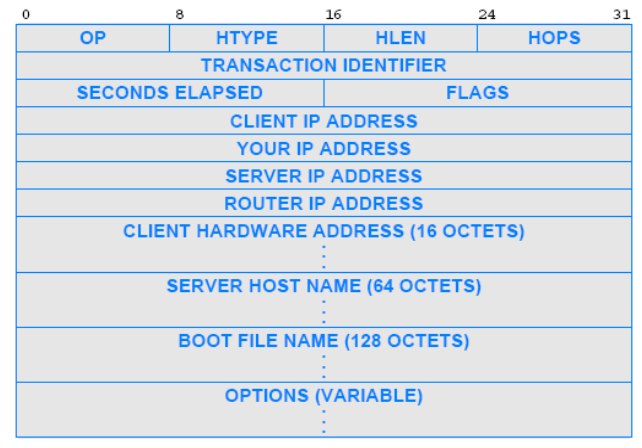
\includegraphics[width=0.5\textwidth]{04/dhcp-message.png}
                \caption{Formato dei messaggi \texttt{DHCP}}
            \end{figure}
            
            Vediamo ora a cosa servono i principali parametri:
            \begin{description}
                \item[\texttt{OP}] Campo di 1 byte che indica se il messaggio è un \textit{request} o un \textit{reply}
                \item[\texttt{HTYPE} e \texttt{HLEN}] Campi di 1 byte l'uno specificano il tipo di \textit{hardware} e la lunghezza dell'indirizzo \texttt{MAC}
                \item[\texttt{FLAGS}] Campo di 2 byte che contiene, ad esempio, se il mittente può ricevere \textit{broadcast} o solo risposte dirette
                \item[\texttt{HOPS}] Campo di 1 byte che indica quanti \textit{server} hanno inoltrato la risposta
                \item[\texttt{TRANSACTION IDENTIFIER}] Campo di 4 byte che identifica la transazione
                \item[\texttt{SECONDS ELAPSED}] Campo di 2 byte che indica da quanto tempo il \textit{client} è in attesa
                \item[\textit{altri}] Ci sono altri campi che indicano l'indirizzo \texttt{IP} del \textit{client}, l'indirizzo \texttt{IP} del \textit{server}, l'indirizzo \texttt{IP} del \textit{router} e l'indirizzo \texttt{IP} del \textit{DNS}.
            \end{description}
        \subsubsection{Se non c'è un \textit{server} \texttt{DHCP}}
            Se non c'è un \textit{server} \texttt{DHCP} allora ci sono due situazioni: la prima è si configura un indirizzo \texttt{IP} statico, mentre, se non riceviamo risposta dopo un certo periodo di tempo, l'\textit{host} provvede all'impostazione di un indirizzo \textit{link-local} che permette la comunicazione con altri \textit{host} nella stessa rete che hanno lo stesso problema.
            \paragraph{Configurazione \textit{link-local}} Per configurare un indirizzo \textit{link-local} si seguono i seguenti passi: \begin{enumerate}
                \item Si sceglie un indirizzo \texttt{IP} compreso tra \texttt{169.254.0.1} e \texttt{169.254.255.254} con maschera di rete \texttt{/16}
                \item Si cerca se esiste una interfaccia di rete con un indirizzo \texttt{IP} \textit{link-local} scelto (tramite \texttt{ARP})
                \item[3.a.] Se esiste un'altra interfaccia con lo stesso indirizzo \texttt{IP} allora si ripete il processo
                \item[3.b.] Altrimenti si configura l'indirizzo \texttt{IP} \textit{link-local}
            \end{enumerate}
    \subsection{Il viaggio di un pacchetto}
        Analizziamo ora il viaggio di un pacchetto da un \textit{host} \texttt{A} ad un \textit{host} \texttt{B} in una rete. assumiamo che \texttt{A} conosca l'indirizzo \texttt{IP} di \texttt{B} e l'indirizzo \texttt{UP} del router \texttt{R} (che è il \textit{default gateway}) (Tramite \texttt{DHCP}), inoltre conosce già l'indirizzo \texttt{MAC} del router \texttt{R} (Tramite \texttt{ARP}).\newline
        Quindi in una rete costituita da \texttt{A}, \texttt{R} e \texttt{B}, con \texttt{R} nel mezzo, il pacchetto viaggia in questo modo: \begin{enumerate}
            \item \texttt{A} crea il datagramma \texttt{IP} con sorgente \texttt{A} e destinazione \texttt{B}
            \item \texttt{A} incapsula il datagramma in un frame di livello 2 con indirizzo \texttt{MAC} di \texttt{R} come destinazione e \texttt{MAC} di \texttt{A} come sorgente
            \item Il frame viene inviato alla rete da \texttt{A} a \texttt{R}\footnote{\label{netSwitch}
                In questo punto possono essere presenti all'interno della rete altri dispositivi di livello 2 come \textit{switch} che inoltrano il pacchetto in base all'indirizzo \texttt{MAC}}
            \item Il frame arriva a \texttt{R} che estrae il datagramma \texttt{IP} e lo passa al livello 3
            \item \texttt{R} controlla la tabella di routing e inoltra il pacchetto a \texttt{B}, per fare ciò incapsula il datagramma in un frame con indirizzo \texttt{MAC} di \texttt{B} come destinazione e \texttt{MAC} di \texttt{R} come sorgente
            \item Il frame viene inviato da \texttt{R} a \texttt{B}\footref{netSwitch}
            \item \texttt{B} estrae il datagramma \texttt{IP} e lo passa al livello 3 per l'elaborazione
        \end{enumerate}
    \subsection{\texttt{IPv6}}
        Il protocollo \texttt{IPv6} è un protocollo nato per ampliare la quantità di indirizzi \texttt{IP} disponibili rispetto quelli di \texttt{IPv4}, successivamente si è voluto standardizzarlo anche in quanto il formato dell'\textit{header} velocizza l'elaborazione dei frammenti, inoltre facilita la gestione della qualità del servizio.\subsubsection{Formato del datagramma \texttt{IPv6}}
            Il formato di un frammento è: \textbf{header} da $40$ byte e la frammentazione è proibita.
            \paragraph{Header} L'\textit{header} di un datagramma \texttt{IPv6} è composto da: \begin{itemize}
                \item \textbf{Flow label} Campo di $20$ bit che permette di identificare un flusso di dati.
                \item \textbf{Priority} Campo di $4$ bit che permette di identificare la priorità del pacchetto.
                \item \textbf{Next header} Campo di $8$ bit che permette di identificare il protocollo di trasporto.
            \end{itemize}
        \subsubsection{Cambiamenti rispetto \texttt{IPv4}}
            In quanto la rete è diventata più affidabile è stato rimosso il \textit{checksum}, vengono rimosse le \textit{options} e il \textit{header} è più corto. Inoltre viene introdotto il protocollo \textit{ICMPv6} con più funzionalità rispetto a \textit{ICMP}.
        \subsubsection{Transizione da \texttt{IPv4} a \texttt{IPv6}}
            La transizione da \texttt{IPv4} a \texttt{IPv6} è molto lenta in quanto richiede un cambiamento di infrastruttura molto grande, per questo si è deciso che se un pacchetto \texttt{IPv6} deve transitare obbligatoriamente per una rete \texttt{IPv4} allora il pacchetto viene incapsulato in un pacchetto \texttt{IPv4} e poi inviato alla rete \texttt{IPv4} e poi riconvertito in un pacchetto \texttt{IPv6} alla destinazione.
        \subsubsection{Indirizzi \texttt{IPv6}}
            La lunghezza non permette notazione \textit{dotted decimal} e quindi si usa la notazione esadecimale: Ogni gruppo di $4$ bit è scritto come una cifra $0,1,\dots,9$ o una lettera: $a,b,\dots,f$. In totale $32$ cifre esadecimali costituiscono un indirizzo \texttt{IPv6}.
            \paragraph{Esempio} Un indirizzo di esempio è \texttt{2a03:2880:f108:0083:face:b00c:0000:25de} che è un indirizzo \texttt{IPv6} valido.
            \paragraph{Raggruppamento} Si possono raggruppare $0$ o omettendoli oppure se è un intero gruppo di $0$ si può omettere tutto il gruppo. Ad esempio l'indirizzo \texttt{2a03:2880:f108:0083:face:b00c:0000:25de} può essere scritto come\texttt{2a03:2880:f108:83:face:b00c:0:25de}. 
        \subsubsection{Indirizzi speciali}
            Gli indirizzi speciali di \texttt{IPv6} sono: \begin{itemize}
                \item \textbf{Unspecified address} Indirizzo $0:0:0:0:0:0:0:0$ che indica che l'indirizzo non è assegnato.
                \item \textbf{Loopback address} Indirizzo $0:0:0:0:0:0:0:1$ che indica l'indirizzo di \textit{loopback}.
                \item \textbf{Link-local address} Indirizzo $fe80::/10$ che indica un indirizzo di \textit{link-local}.
                \item \textbf{Site-local address} Indirizzo $fec0::/10$ che indica un indirizzo di \textit{site-local}.
                \item \textbf{Multicast address} Indirizzo $ff00::/8$ che indica un indirizzo di \textit{multicast}.
            \end{itemize}
\section{Protocolli di instradamento}
    I protocolli di instradamento sono protocolli che permettono la creazione di una tabella di \textit{routing} per instradare i pacchetti da un \textit{host} ad un altro tramite il miglior percorso possibile. Un "buon percorso" è definito in base a diversi fattori come: il "costo" più basso, la "velocità" più alta il percorso meno congestionato. 
    \paragraph{Modello a Grafo} Possiamo rappresentare una rete come un grafo, dove i nodi sono i \textit{router} e gli archi sono i collegamenti tra i \textit{router}. Ad ogni arco è associato un "costo" di trasmissione di un pacchetto da un \textit{router} all'altro. Il costo potrebbe essere: il numero di salti, la banda del link (proporzionale al costo monetario), l'inverso della banda, la congestione del link o l'algoritmo usato. Per il calcolo di un costo tra più router si sommano i costi di ogni arco.
    \paragraph{Tipi di routing}
        I protocolli di instradamento possono essere classificati in due categorie: \begin{itemize}
            \item \textbf{Routing statico} Il percorso è definito manualmente dall'amministratore di rete. Questo percorso non cambia se non manualmente.
            \item \textbf{Routing dinamico} Le rotte cambiano più frequentemente sulla base di aggiornamenti periodici e tipicamente a causa di cambiamenti nel costo dei collegamenti.
        \end{itemize}
        Le informazioni su questo tipo di cambiamenti può essere globale o distribuita.
        \begin{itemize}
            \item \textbf{Routing globale} Tutti i \textit{router} conoscono la topologia della rete e i costi di trasmissione.
            \item \textbf{Routing distribuito} I \textit{router} conoscono solo i costi dei collegamenti diretti ai quali sono collegati, il processo di calcolo è iterativo e distribuito (uso di algoritmi \textit{distance-vector}).
        \end{itemize}
    \subsection{\textit{Link State} "Dijkstra"}
        Nell'algoritmo di \textit{Dijkstra} si assume che la topologia di rete e i costi dei link, siano noti a tutti i \textit{router}. Allora in output otteniamo il percorso a costo minimo. Inoltre l'algoritmo è iterativo in quanto dopo $k$ iterazioni si conosce il percorso a costo minimo verso $k$ destinazioni.\newline
        Viene usata la seguente notazione: \begin{itemize}
            \item $c(x,y)$ costo del collegamento tra $x$ e $y$
            \item $D(v)$ costo del percorso a costo minimo verso $v$
            \item $p(v)$ nodo precedente di $v$ lingo il cammino dalla sorgente a $v$
            \item $N'$ insieme dei nodi per cui il cammino a costo minimo è già stato trovato
        \end{itemize}\newpage
        L'algoritmo funziona in questo modo:

        \begin{algorithm}[H]
            \SetAlgoLined
            \textbf{Inizializzazione:}\;
            $N' \gets \{u\}$ \tcp*[f]{\textcolor{orange}{nodo corrente}} \;
            \ForEach{nodo $v$}{
                \eIf{$v$ è adiacente a $u$}{
                    $D(v) \gets c(u, v)$\;
                    $p(v) \gets u$\;
                }{
                    $D(v) \gets \infty$\;
                }
            }
            \textbf{Loop:}\;
            \While{tutti i nodi non sono contenuti in $N'$}{
                Trova $w \notin N'$ tale che $D(w)$ è minimo\;
                Aggiungi $w$ a $N'$\;
                \ForEach{nodo $v$ adiacente a $w$ e $v \notin N'$}{
                    \If{$D(w) + c(w, v) < D(v)$}{
                        $D(v) \gets D(w) + c(w, v)$\;
                        $p(v) \gets w$\;
                    }
                }
            }
            \tcp*[f]{\textcolor{orange}{Il nuovo costo verso $v$ è il costo già noto, oppure il costo minimo verso $w$ più il costo da $w$ a $v$}} \;
            \caption{Algoritmo per la ricerca dei percorsi minimi}
        \end{algorithm}
        Come si può notare il seguente algoritmo costruisce i percorsi minimi tracciando a ritroso i nodi predecessori, possono esserci più percorsi minimi tra due nodi in questo caso se ne sceglie uno a caso.
        \paragraph{Complessità dell'algoritmo} L'algoritmo di \textit{Dijkstra} con una rete di $n$ nodi deve controllare ad ogni iterazione tutti i nodi tale che $w\neq N'$ dunque questo tende a: $ \frac{n(n+1)}2$ operazioni, quindi la complessità è $O(n^2)$. Esistono però algoritmi di complessità $O(n\log n)$. 
    \subsection{Internet, \texttt{AS}, \texttt{OSPF}}
        Internet è una rete di reti, ognuna di queste reti è proprietà di un'organizzazione quale un \texttt{ISP}, un operatore di rete, una azienda o anche uno stato. Ogni rete idealmente dovrebbe avere due Caratteristiche importanti: \begin{itemize}
            \item \textbf{Autonomia} Ogni rete dovrebbe essere amministrativamente autonoma e avere il controllo della propria politica di instradamento.
            \item \textbf{Connessione} Ogni rete dovrebbe essere in grado di collegarsi ad ognuna delle altre reti.
        \end{itemize}
        Da queste necessità vengono creati gli \texttt{AS} (\textit{Autonomous System}) i quali vengono definiti come: "Un gruppo di \textit{router} sotto lo stesso controllo amministrativo", ognuno di questi \texttt{AS} è identificato da un numero univoco chiamato \texttt{ASN} (\textit{Autonomous System Number}) assegnato da un ente chiamato \texttt{ICANN} (\textit{Internet Corporation for Assigned Names and Numbers}). \newline
        Nasce ora la necessità di definire degli algoritmi di \textbf{Intra-\texttt{AS}} e \textbf{Inter-\texttt{AS}}. Per l'\textit{Intra-\texttt{AS}} intendiamo l'instradamento all'interno di un \texttt{AS}, mentre per l'\textit{Inter-\texttt{AS}} intendiamo l'instradamento tra due \texttt{AS} differenti.
        \subsubsection{Intra-\texttt{AS}: \textit{Open Shortest Path First} (\texttt{OSPF})}
            Il protocollo \texttt{OSPF} è un protocollo di instradamento Intra-\texttt{AS} basato su \textit{link-state}, questo protocollo è basato sull'assunzione che ogni router che lo applica conosca tutta la topologia della rete. Per il funzionamento sfrutta dei datagramma \texttt{IP} senza servirsi del livello di trasporto, in quanto la comunicazione deve essere inviata a tutti i router sfrutta l'indirizzo \texttt{IP} di \textit{broadcast} \texttt{224.0.0.5}.
            \paragraph{Procedure} Il protocollo \texttt{OSPF} implementa tre procedure: \begin{itemize}
                \item Protocollo "\texttt{Hello}" - I \textit{router} si scambiano messaggi di mantenimento per controllare il corretto funzionamento del link e dei nodi ad esso collegati.
                \item Protocollo "\texttt{Exchange}" - I \textit{router} si scambiano informazioni di \textit{link-state} sulla topologia della rete al momento conosciuta.
                \item Protocollo "\texttt{Flooding}" - I \textit{router} inviano i messaggi di \textit{link-state} a tutti i \textit{router} della rete contenenti un cambio di stato di un \textit{link}.
            \end{itemize}
            \subparagraph{\textit{Flooding} controllato} Normalmente in caso di \textit{flooding} quando un router riceve un messaggio di questo genere provvede a inoltrarlo a tutti i suoi vicini: in reti del genere \texttt{/30} tramite un messaggio diretto, in tutte le altre reti tramite \textit{broadcast}. In questo modo si evitano inutili repliche di messaggi.
        \paragraph{\texttt{OSPF} gerarchico} Generalmente un router potrebbe non voler conoscere tutta la topologia della rete, ma solo una parte di essa. Per questo motivo si è deciso di instaurare una gerarchia a due livelli: \begin{itemize}
            \item \textbf{Dorsale} (\textit{Backbone}) Questo livello è costituito da \textit{router} che conoscono tutta la topologia della rete.
            \item \textbf{Area} Questo livello è costituito da \textit{router} che conoscono solo la topologia della propria area, ma sanno che esiste un percorso tramite un router di bordo\footnote{Da \underline{\textbf{NON}} confondere con il \textit{router} di confine \texttt{AS}} per raggiungere un'altra area.
        \end{itemize}
        La dorsale oltre a conoscere tutta la topologia della rete, è considerata anche come "area" infatti questa non fà girare i messaggi di \texttt{OSPF} al di fuori di essa, se non per i \textit{router} di bordo.
        \paragraph{Gestione dei costi} \texttt{OSPF} è un protocollo \textit{link-state} dunque l'unica cosa della quale si tiene consto è il costo del collegamento e non altri fattori esterni. Alcuni operatori potrebbero agire sul costo dei \textit{link} per influenzare il percorso dei pacchetti.
    \subsection{Routing con \textit{distance vector}: \textit{Bellman-Ford}}
        L'algoritmo di \textit{Bellman-Ford} è un algoritmo di instradamento che permette di trovare il percorso a costo minimo senza dover conoscere l'intera tipologia di rete, richiede però che ogni nodo conosca i suoi "vicini" e il coso del \textit{link} che li collega. L'eventuale presenza di ulteriori nodi che non siano i vicini viene notificata tramite messaggi.
        \paragraph{Notazione} \begin{itemize}
            \item $N$: insieme di vicini $\Rightarrow N_x$ i vicini del \textit{router} $x$
            \item $R$: tabella di \textit{routing} $\Rightarrow R_x$ la tabella di \textit{routing} del \textit{router} $x$
                \subitem $R[d]$ riga della tabella di \textit{routing} che contiene le informazioni per raggiungere il nodo $d$, $R[d].\operatorname{cost}$ il costo per raggiungere il nodo $d$ e $R[d].\operatorname{nexthop}$ il prossimo nodo per raggiungere il nodo $d$, $R[d].\operatorname{time}$ il tempo dell'ultima modifica.
            \item $D$ vettore con tutte le distanze $\Rightarrow D_x$ il \textit{distance vector} del \textit{router} $x$
                \subitem $D_x=[<d,R_x[d].\operatorname{cost}>]$ tale che $d\in R_x$
        \end{itemize}
        \paragraph{Algoritmo} L'algoritmo funziona in questo modo:

            \begin{algorithm}[H]
                \SetAlgoLined
                \textbf{Inizializzazione:}\;
                Per tutte le destinazioni $y \rightarrow D_x(y) = c(x,y)$\;
                Per tutti i vicini $w$, e tutte le destinazioni $y \rightarrow D_w(y) = ?$\;
                Per ogni vicino $w \rightarrow \text{invia } D_x = [D_x(y):y\in N_x] \text{ a } w$\;
                \textbf{Loop:}\;
                Aspetto finché il costo verso in vicino non cambia o non ricevo $D_w$ da un vicino $w$\;
                \ForEach{destinazione $y$}{
                    $D_x(y) = \min_v \{c(x,v) + D_v(y)\}$\;
                    $\operatorname{nexthop}_x(y) = \operatorname{argmin}_v \{c(x,v) + D_v(y)\}$\;
                }
                \If{$D_x(y)$ cambia per qualche $y$}{
                    \ForEach{vicino $w$}{
                        \text{invia } $D_x = [D_x(y):y\in N_x] \text{ a } w$\;
                    }
                }
                \caption{Algoritmo di \textit{Bellman-Ford}}
            \end{algorithm}
        \paragraph{\textit{Count to infinity}} Un problema che si può presentare in questo algoritmo è il problema del \textit{count to infinity}, ovvero il problema che al momento di una interruzione di un collegamento si potrebbero creare \textit{loop} di instradamento. Andando quindi a rendere irraggiungibile una destinazione. Vengono quindi adottate delle tecniche per ovviare il problema:
            \subparagraph{Massimo numero di \textit{hop}} Si può decidere di limitare il numero di \textit{hop} per la propagazione dei \texttt{DV}, solitamente si usa $15$ come numero massimo di \textit{hop}. Questa soluzione abbassa il tempo di convergenza ma non elimina il problema.
            \subparagraph{\textit{Split Horizon}} Questa semplice tecnica consiste nell'omissione delle nuove rotte allo stesso nodo da cui sono state ricevute. Più in avanti un esempio di "non funzionamento" di questa tecnica.
            \subparagraph{\textit{Poison Reverse}} Questa soluzione prevede che "Finché un nodo $x$ raggiunge un nodo $z$ passando per $y$ allora $x$ comunica a $y$ che $D_x(z)=\infty$". In questo modo il \textit{router} $y$ non cercherà di raggiungere $z$ passando per $x$. Più in avanti un esempio di "non funzionamento" di questa tecnica.
        \paragraph{Cambio di costi} Nel caso in cui il costo di un \textit{link} cambi se questo è in diminuzione, allora la propagazione viaggia velocemente, mentre se il costo è in aumento allora la propagazione viaggia lentamente.
        \paragraph{Caso di non-funzionamento di \textit{split-horizon} e \textit{poisoned reverse}}
        Si prenda in considerazione il seguente esempio:
            \begin{figure}[H]
                \centering
                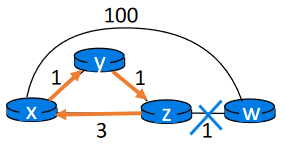
\includegraphics[width=0.4\textwidth]{04/exampleFail.png}
                \caption{Esempio di non funzionamento di \textit{split-horizon} e \textit{poisoned reverse}}
            \end{figure}
        
        Partendo dal presupposto che per raggiungere $W$ il router $X$ abbia \textit{next-hop} a $Y$, $y$ abbia \textit{next-hop} a $Z$ e $Z$ abbia \textit{next-hop} a $W$ in quanto questi sono i collegamenti più convenienti.\newline
        Nel caso di rottura del \textit{link} $Z-W$ allora in quanto i nodi operano in modo distribuito il \textit{router} $X$ potrebbe inviare un pacchetto del tipo: $D_X=[(Y,1),(Z,3)]$ a $Y$ e $D_X=[(W,3),(Y,1),(Z,3)]$ a $Z$. In questo modo $Y$ lascia la sua tabella invariata in quanto già sapeva che $Z$ era il \textit{next-hop} per $W$, mentre $Z$ che ha "perso" il \textit{link} diretto con $W$ non ha nulla sulla sua tabella ed inserisce il che il prossimo \textit{hop} per $W$ è $X$ con costo $6$. Ma $X$ si aspetta di inviare i pacchetti per $W$ a $Y$ il quale li invierà a $Z$ creando un \textit{loop} di instradamento. Questo problema accadrà finché $X$ non si "accorgerà" che il link diretto ma più costoso $X-W$ è il migliore per raggiungere $W$, a quel punto $X$ invierà a $Y$ il pacchetto $D_X=[(Y,1),(Z,3),(W,100)]$. 
    \subsection{Intra-\texttt{AS}: \textit{Routing Information Protocol} (\texttt{RIP})}
        Il protocollo \texttt{RIP} è un protocollo di \textit{routing} Intra-\texttt{AS}, questo implementa \textit{distance vector} ed ha come vantaggio che è semplice da implementare e gestire, d'altra parte è a convergenza lenta e si ha una dimensione limitata della rete.
        \subsubsection{funzionamento} Nel \texttt{RIP} il costo dei link è dato dal numero di \textit{hop} dove $15$ è il numero massimo di salti e da $16$ la distanza è $\infty$ (non raggiungibile) limitando la convergenza. Ogni $30$ secondi poi il protocollo \texttt{RIP} precede di un nuovo invio di \textit{distance vector} (\texttt{DV}) dove ogni messaggio di \textit{\texttt{RIP} advertisement} contiene al massimo $25$ destinazioni all'interno dell'\texttt{AS}, per eseguire lo scambio di messaggi si usa la porta \texttt{UDP} $520$ con indirizzo di destinazione \texttt{224.0.0.9}.
        \subsubsection{In caso di guasto}
            Nel caso un \textit{router} non riceva per $180$ secondi un messaggio di \texttt{RIP} da un \textit{router} vicino allora il \textit{router} considera il collegamento come guasto, andando a modificare la tabella di \textit{routing} e propagando il cambiamento agli altri \textit{router}.
        \subsubsection{Tabella d'instradamento}
            Un processo chiamato \texttt{routed} esegue \texttt{RIP}, ossia un \textit{daemon} che esegue il protocollo \texttt{RIP} e mantiene la tabella di \textit{routing}. 
        \subsubsection{Confronto con \textit{link-state}}
            A livello di complessità di scambio negli algoritmi \textit{link-state} avendo $n$ nodi e $E$ link allora vengono scambiati $O(ne)$ messaggi, mentre in \texttt{RIP} vengono inviati messaggi solo ai vicini e quindi il numero di messaggi scambiati è $O(n)$, ma il tempo di convergenza dipende.\newline
            Per la velocità di convergenza nel caso di \texttt{RIP} e quindi \textit{distance vector} si ha che la convergenza è lenta e si potrebbero avere \textit{loop} di instradamento, mentre in \textit{link-state} la complessità è $O(n^2)$ e quindi la convergenza è più veloce e non si hanno \textit{loop} di instradamento.\newline
            Infine a livello di robustezza si ha che in \texttt{LS} i nodi potrebbero comunicare costi sbagliati per i \textit{link} e spetta al singolo nodo gestire la propria tabella, mentre in \texttt{DV} i nodi comunicano solo con i vicini e quindi si ha una maggiore robustezza ma i nodi potrebbero comunicare costi sbagliati per i percorsi.
    \subsection{\textit{Border Gateway Protocol} (\texttt{BGP})}
        Il protocollo \texttt{BGP} è un protocollo di instradamento Inter-\texttt{AS} che permette di instradare pacchetti tra \textit{AS} differenti. Questo protocollo è stato creato perché i protocolli di instradamento Intra-\texttt{AS} non sono adatti per la scalabilità di internet. Gli \texttt{AS} comunicano tra loro per scambiare informazioni di instradamento e di raggiungibilità, ogni \texttt{AS} decide autonomamente come instradare i pacchetti decidendo inoltre con quali altri \texttt{AS} scambiare informazioni.
        \subsubsection{funzionamento}
            Il protocollo \texttt{BGP} è un protocollo \textit{path vector} che, in quanto le relazioni tra \texttt{AS} possono essere complesse, permette di adattarsi a tutti i possibili casi. Ogni \texttt{AS} è in grado di decidere se: pubblicizzare o meno le proprie informazioni di raggiungibilità, ritirare la raggiungibilità di qualunque rete, offrire o meno transito ad altri \texttt{AS} e filtrare le informazioni di raggiungibilità.\newline
            Ogni \texttt{AS} ha un certo numero di \textit{router} "\texttt{BGP} \textit{speaker}" che scambiano informazioni con i \textit{router} degli altri \texttt{AS} una volta messi in relazione. Questi \textit{speaker} scambiano informazioni su quale è la rete raggiungibile, quale è il prossimo \textit{hop} e quale è il percorso.
            \paragraph{Interconnessioni tra \texttt{AS}} Le interconnessioni tra \texttt{AS} possono essere di due tipi: \begin{itemize}
                \item \textbf{Peering} Due \texttt{AS} si scambiano informazioni di raggiungibilità senza scambiarsi denaro.
                \item \textbf{client - provider} Un \texttt{AS} paga un \textit{provider} per l'accesso a internet.
                \item \textbf{provider - client} il provider viene pagato dal \textit{client} per l'accesso alle informazioni di raggiungibilità.
            \end{itemize}
        \subsubsection{\textit{Best Path} \texttt{BGP}}
            Il \textit{best path} di \texttt{BGP} si differenzia da \texttt{OSPF} e \texttt{RIP} nei quali si preferiva il percorso più breve, in \texttt{BGP} il percorso migliore dipende dalle \textit{policy} degli \texttt{AS} e non dal costo del percorso. Un cambiamento di \textit{policy} dovuto a delle modifiche economiche di contratto potrebbe portare alla modifica del percorso per altri \texttt{AS} oltre a quello che ha cambiato la \textit{policy}.\newline
            Considerando questi fattori imo \textit{speaker} \texttt{BGP} condivide solamente la sua \textit{best path} con gli altri \textit{speaker} \texttt{BGP}, se uno \textit{speaker} decide di ignorare una altro percorso allora non lo comunica, ciò potrebbe comportare a delle destinazioni irraggiungibili se un terzo \textit{AS} ha politiche in conflitto con la rotta comunicata da un altro \textit{AS}.
            
        \subsubsection{Messaggi \texttt{BGP}}
            Il protocollo \texttt{BGP} usa 4 messaggi:
            \paragraph{\texttt{OPEN}} Messaggio di apertura di una connessione \texttt{BGP}, se il messaggio viene accettato allora si invia un messaggio \texttt{KEEPALIVE} di conferma, alla ricezione la connessione è aperta. All'interno di un messaggio \texttt{OPEN} viene inviato il numero di versione, l'\texttt{ASN} del mittente, il tempo di \textit{hold} che viene prima proposto da chi apre la connessione e poi confermato o confermato con un valore più altro oppure viene rifiutato rispondendo con un tempo minore. Viene inviato con il messaggio di apertura anche il \texttt{BGP Identifier} che è l'identificativo univoco dello speaker \texttt{BGP}, uguale per tutte le sue interfacce \texttt{BGP}.
            \paragraph{\texttt{NOTIFICATION}} Messaggio di errore con $6$ possibili codici di errore relativi al tipo di questo, $20$ possibili sottotipi in base a dove l'errore si presenta. 
            \paragraph{\texttt{KEEPALIVE}} Messaggio di conferma di ricezione, inviato ogni $x$ secondi per mantenere la connessione aperta, questo messaggio non contiene dati ma solo un \textit{header} di $19$ byte.
            \paragraph{\texttt{UPDATE}} Messaggio più complesso, contiene le informazioni di raggiungibilità, il percorso e le \textit{policy} di instradamento. Questo messaggio può contenere informazioni del tipo: \texttt{Additive}, quando nuove informazioni vengono aggiunte, \texttt{Sottrattive} quando informazioni vengono rimosse.
                \subparagraph{\texttt{WITHDRAW}} Questo tipo di messaggio viene inviato quando un percorso viene rimosso, in questo caso il messaggio contiene solo l'identificativo del percorso rimosso. Questo messaggio viene inviato in caso di \textit{link} guasti o di cambiamenti di \textit{policy} e solo se questi cambiamenti comportano la irraggiungibilità di un \texttt{AS} da parte di chi invia il messaggio.
                \subparagraph{\texttt{UPDATE + WITHDRAW}} Questi messaggi vengono inviati quando un percorso viene rimosso e ne viene aggiunto un altro, in questo caso viene prima inviato il messaggio di \texttt{WITHDRAW} contenente il percorso rimosso e poi il messaggio di \texttt{UPDATE} contenente il nuovo percorso.
                \subparagraph{\textit{Implicit} \texttt{WITHDRAW}} Questo tipo di messaggio viene inviato quando un percorso viene rimosso e viene aggiunto un altro percorso, in questo caso il messaggio contiene solo il nuovo percorso. Piccola nota a margine solo alcuni \textit{speaker} \texttt{BGP} supportano questo tipo di messaggio.
        \subsubsection{Aggregazione delle rotte}
            In quanto un \texttt{AS} potrebbe essere il \textit{best path} per più \texttt{AS} differenti questo potrebbe decidere di aggregare le rotte per ridurre il numero di rotte pubblicizzate. In questo modo il \texttt{AS} invia solo una rotta per raggiungere un insieme di \texttt{AS}, questa viene pubblicizzata come una qualsiasi combinazione degli \texttt{AS} raggiungibili. Questo permette di ridurre il numero di rotte pubblicizzate e quindi di ridurre il carico sui \textit{router} e sui \textit{link}.
        \subsubsection{Filtri}
            I \texttt{BGP} \textit{speaker} possono filtrare le informazioni che entrano e/o escono da questi, possono essere filtri specifici del tipo: \texttt{Ingress filters} o \texttt{Egress filters} che permettono di filtrare le informazioni in entrata o in uscita, possono anche esserci però filtri generici che permettono di bloccare "tutto ciò che contenga $X$". Questi filtri possono essere molto o poco precisi e possono essere usati per bloccare informazioni di raggiungibilità o per bloccare informazioni di \textit{policy}.
        \subsubsection{\textit{Routing Information Base} (\texttt{RIB})}
            Le informazioni sulle rotte devono essere in qualche modo conservate sul \textit{router}, queste informazioni vengono conservate nella \texttt{RIB} che, costituita da 3 tabelle, contiene le informazioni di raggiungibilità accettate (\texttt{ADJ\_RIB\_IN}), le informazioni su quelle che vengono attualmente usate (\texttt{LOC\_RIB}) e le informazioni che vengono pubblicizzate (\texttt{ADJ\_RIB\_OUT}). Queste tabelle vengono modificate sulla base di messaggi \texttt{BGP} ricevuti e di \textit{policy} impostate.
            \paragraph{Ricezione di un \texttt{UPDATE}} Se il pacchetto ricevuto viene approvato dai filtri in ingresso, allora questa nuova rotta viene aggiunta alla tabella \texttt{ADJ\_RIB\_IN}, viene quindi ri-valutata la \textit{best path} sulla base delle nuove aggiornate informazioni, nel caso in cui la nuova rotta sia migliore di quella attuale allora viene aggiornata la tabella \texttt{LOC\_RIB} poi se i filtri lo permettono viene aggiornata la tabella \texttt{ADJ\_RIB\_OUT} e inoltrati i cambiamenti ai \textit{router} vicini. Nel caso in cui la nuova rotta sia peggiore di quella attuale allora viene comunque tenuta in memoria per eventuali cambiamenti futuri ma non viene ne aggiornata la tabella \texttt{LOC\_RIB} ne la tabella \texttt{ADJ\_RIB\_OUT} e quindi non viene inoltrata ai \textit{router} vicini.
            \paragraph{Ricezione di un \texttt{WITHDRAW}} Se un \textit{router} riceve un messaggio di \texttt{WITHDRAW} e questo soddisfa i filtri di ingresso, allora le informazioni relative al percorso vengono rimosse dalla tabella \texttt{ADJ\_RIB\_IN} e quindi viene ri-valutata la \textit{best path} e aggiornata, eventualmente, la tabella \texttt{LOC\_RIB} e la tabella \texttt{ADJ\_RIB\_OUT} diffondendo i cambiamenti ai \textit{router} vicini, se ve ne sono.
        \subsubsection{\texttt{BGP} all'interno di \texttt{AS} - \texttt{iBGP}}
            Un grande \texttt{AS} potrebbe avere diversi \textit{router} che agiscono da \textit{speaker} \texttt{BGP}, in quanto \texttt{BGP} si occupa di instradare i pacchetti attraverso \texttt{AS} non si distingue tra quali router devo passare. Per questo motivo si è deciso di creare un protocollo di \textit{routing} interno all'\texttt{AS} chiamato \texttt{iBGP} che permette di scambiare informazioni tra i \textit{router} dello stesso \texttt{AS} e di mantenere aggiornate le tabelle di \textit{routing} all'interno dell'\texttt{AS} in modo da poter instradare i pacchetti che provengono da un \texttt{AS} esterno e devono essere instradati verso un altro \texttt{AS} esterno.
        \paragraph{In caso di più rotte} Nel caso un \textit{router} interno ad un \texttt{AS} abbia la possibilità di passare per rotte diverse per raggiungere un \texttt{AS} esterno allora tramite \texttt{iBGP} i \textit{router} interni possono scambiarsi informazioni e decidere quale percorso è il migliore per raggiungere l'\texttt{AS} esterno. Esempio: considerando gli \texttt{AS}: \texttt{AS1}, \texttt{AS2}, \texttt{AS3} i quali contengono tutti i router \texttt{xA}, \texttt{xB}, \texttt{xC} e \texttt{xD} con i \textit{router} interni collegati a maglia completa\footnote{Tutti i \textit{router} sono collegati a tutti gli altri internamente} e i \textit{router} esterni collegati come segue: \texttt{1C-2A}, \texttt{1C-3A}, \texttt{3A-2C} e \texttt{3D-X}\footnote{Considerando \texttt{X} una altra rete esterna}. Allora i router interni \texttt{2B} e \texttt{2D} avranno la possibilità di raggiungere la rete \texttt{X} sia tramite $[2[B\mid D],2A,1C,3A,3D,X]$ che tramite $[2[B\mid D],2C,3A,3D,X]$ la scelta del percorso migliore verrà fatta tramite politiche interne all'\texttt{AS} e tramite il protocollo \texttt{iBGP}.\newline
        Figura di riferimento: \ref{fig:reteAS-iBGP}
        \begin{figure}[H]
            \centering
            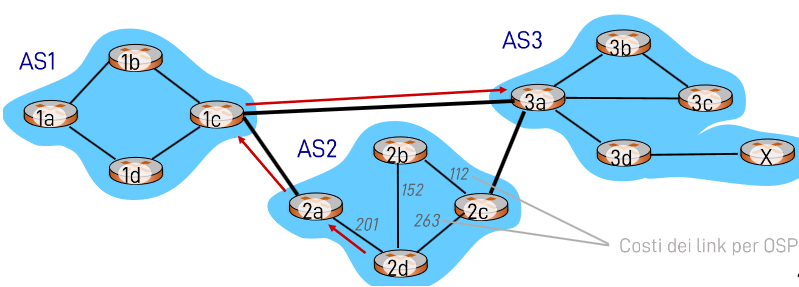
\includegraphics[width=0.6\textwidth]{04/reteAS-iBGP.png}
            \caption{Esempio di rete con \texttt{iBGP} e scelta di percorso}
            \label{fig:reteAS-iBGP}
        \end{figure}
    \subsection*{Riassumendo}
        \begin{itemize}
            \item Gli \texttt{AS} sono interconnessi tra loro e comunicano informazioni di raggiungibilità tramite il protocollo \texttt{BGP}.
            \item Gli \texttt{AS} formano un grafo gerarchico e possono essere di solo transito
            \item Ogni \texttt{AS} è autonomo per definizione (\textit{\textbf{\underline{Autonomous}  System}})
            \item Il \textit{\textbf{Best Path}} di \texttt{BGP} è determinato dalle \textit{policy} degli \texttt{AS} ed non è per forza il percorso più breve. (Politiche economiche, commerciali, estere possono influenzare il percorso)
            \item \texttt{BGP} è un protocollo \textit{path vector} e non \textit{distance vector}, condivide il percorso ma non il costo e/o la distanza.
            \item \texttt{BGP} può contenere diversi filtri sulla base di \textit{policy} e di raggiungibilità.
        \end{itemize}